\chapter{预备知识}\label{sec:preliminaries}
\begin{figure}[t]
    \centering
	\begin{subfigure}[b]{0.48\linewidth}
		\centering
		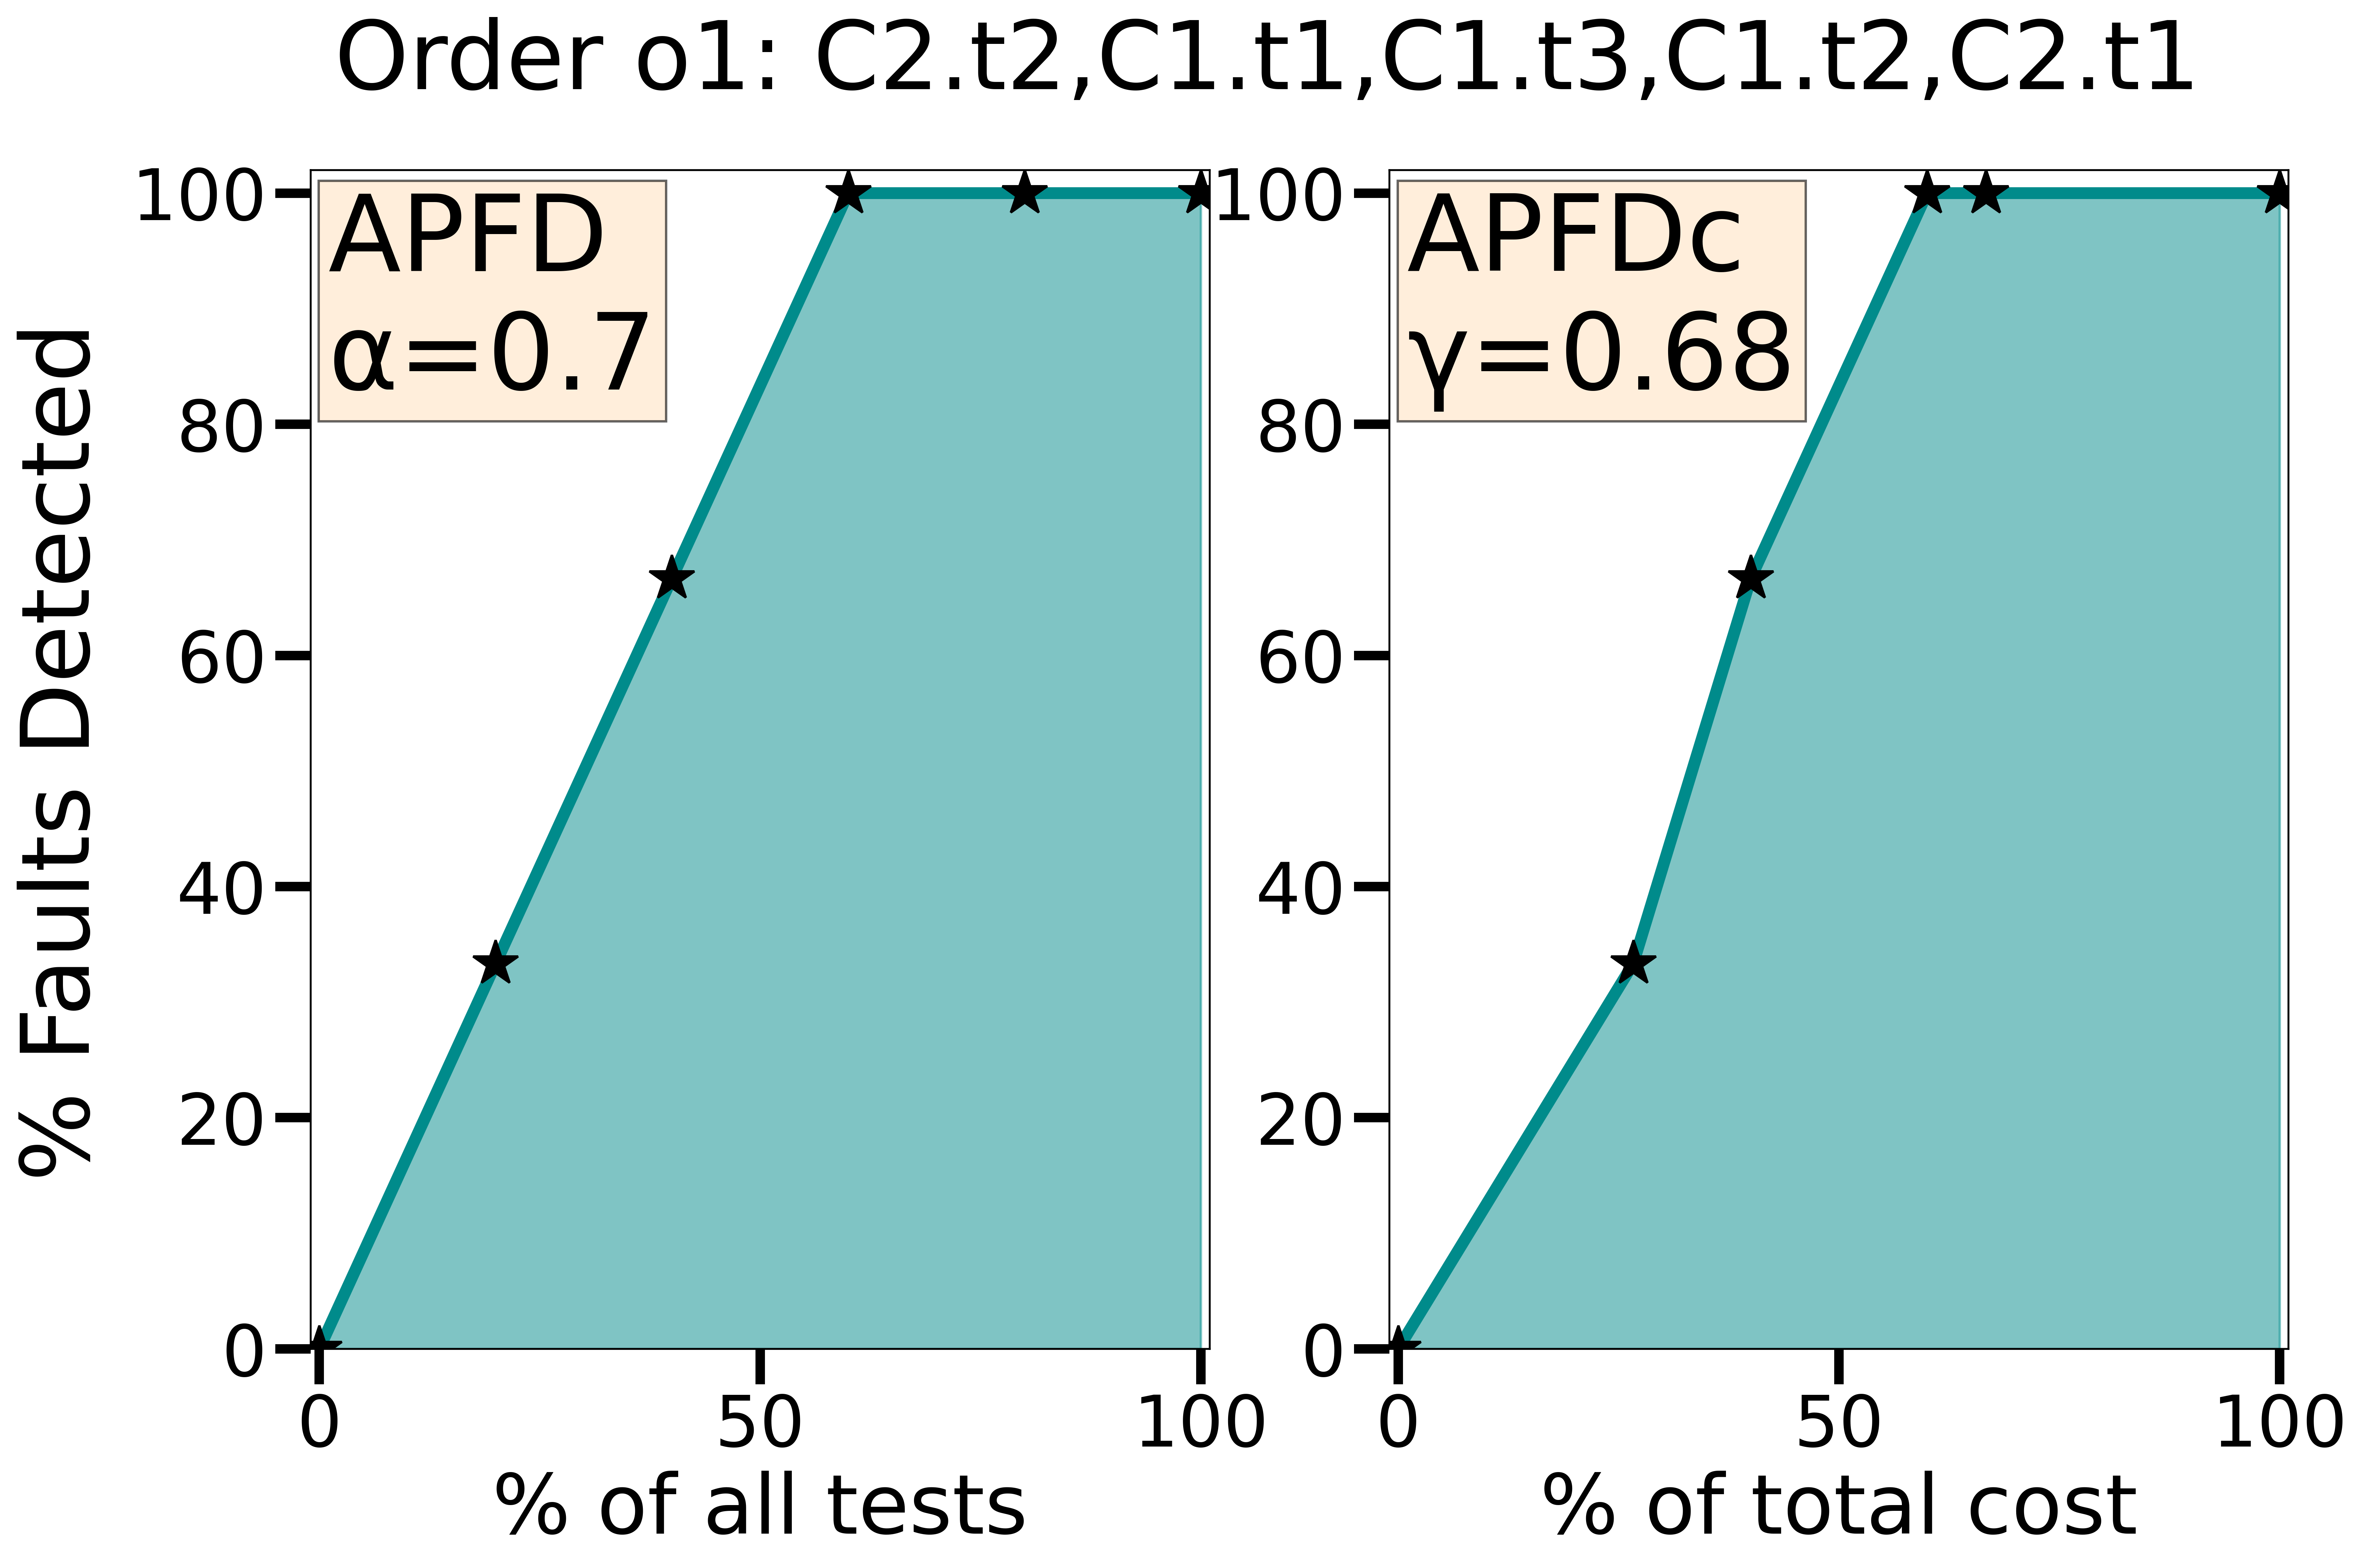
\includegraphics[width=\textwidth]{figures/5-1-3-2-4.png}
	\end{subfigure}
	\hfill
	\begin{subfigure}[b]{0.48\linewidth}
		\centering
		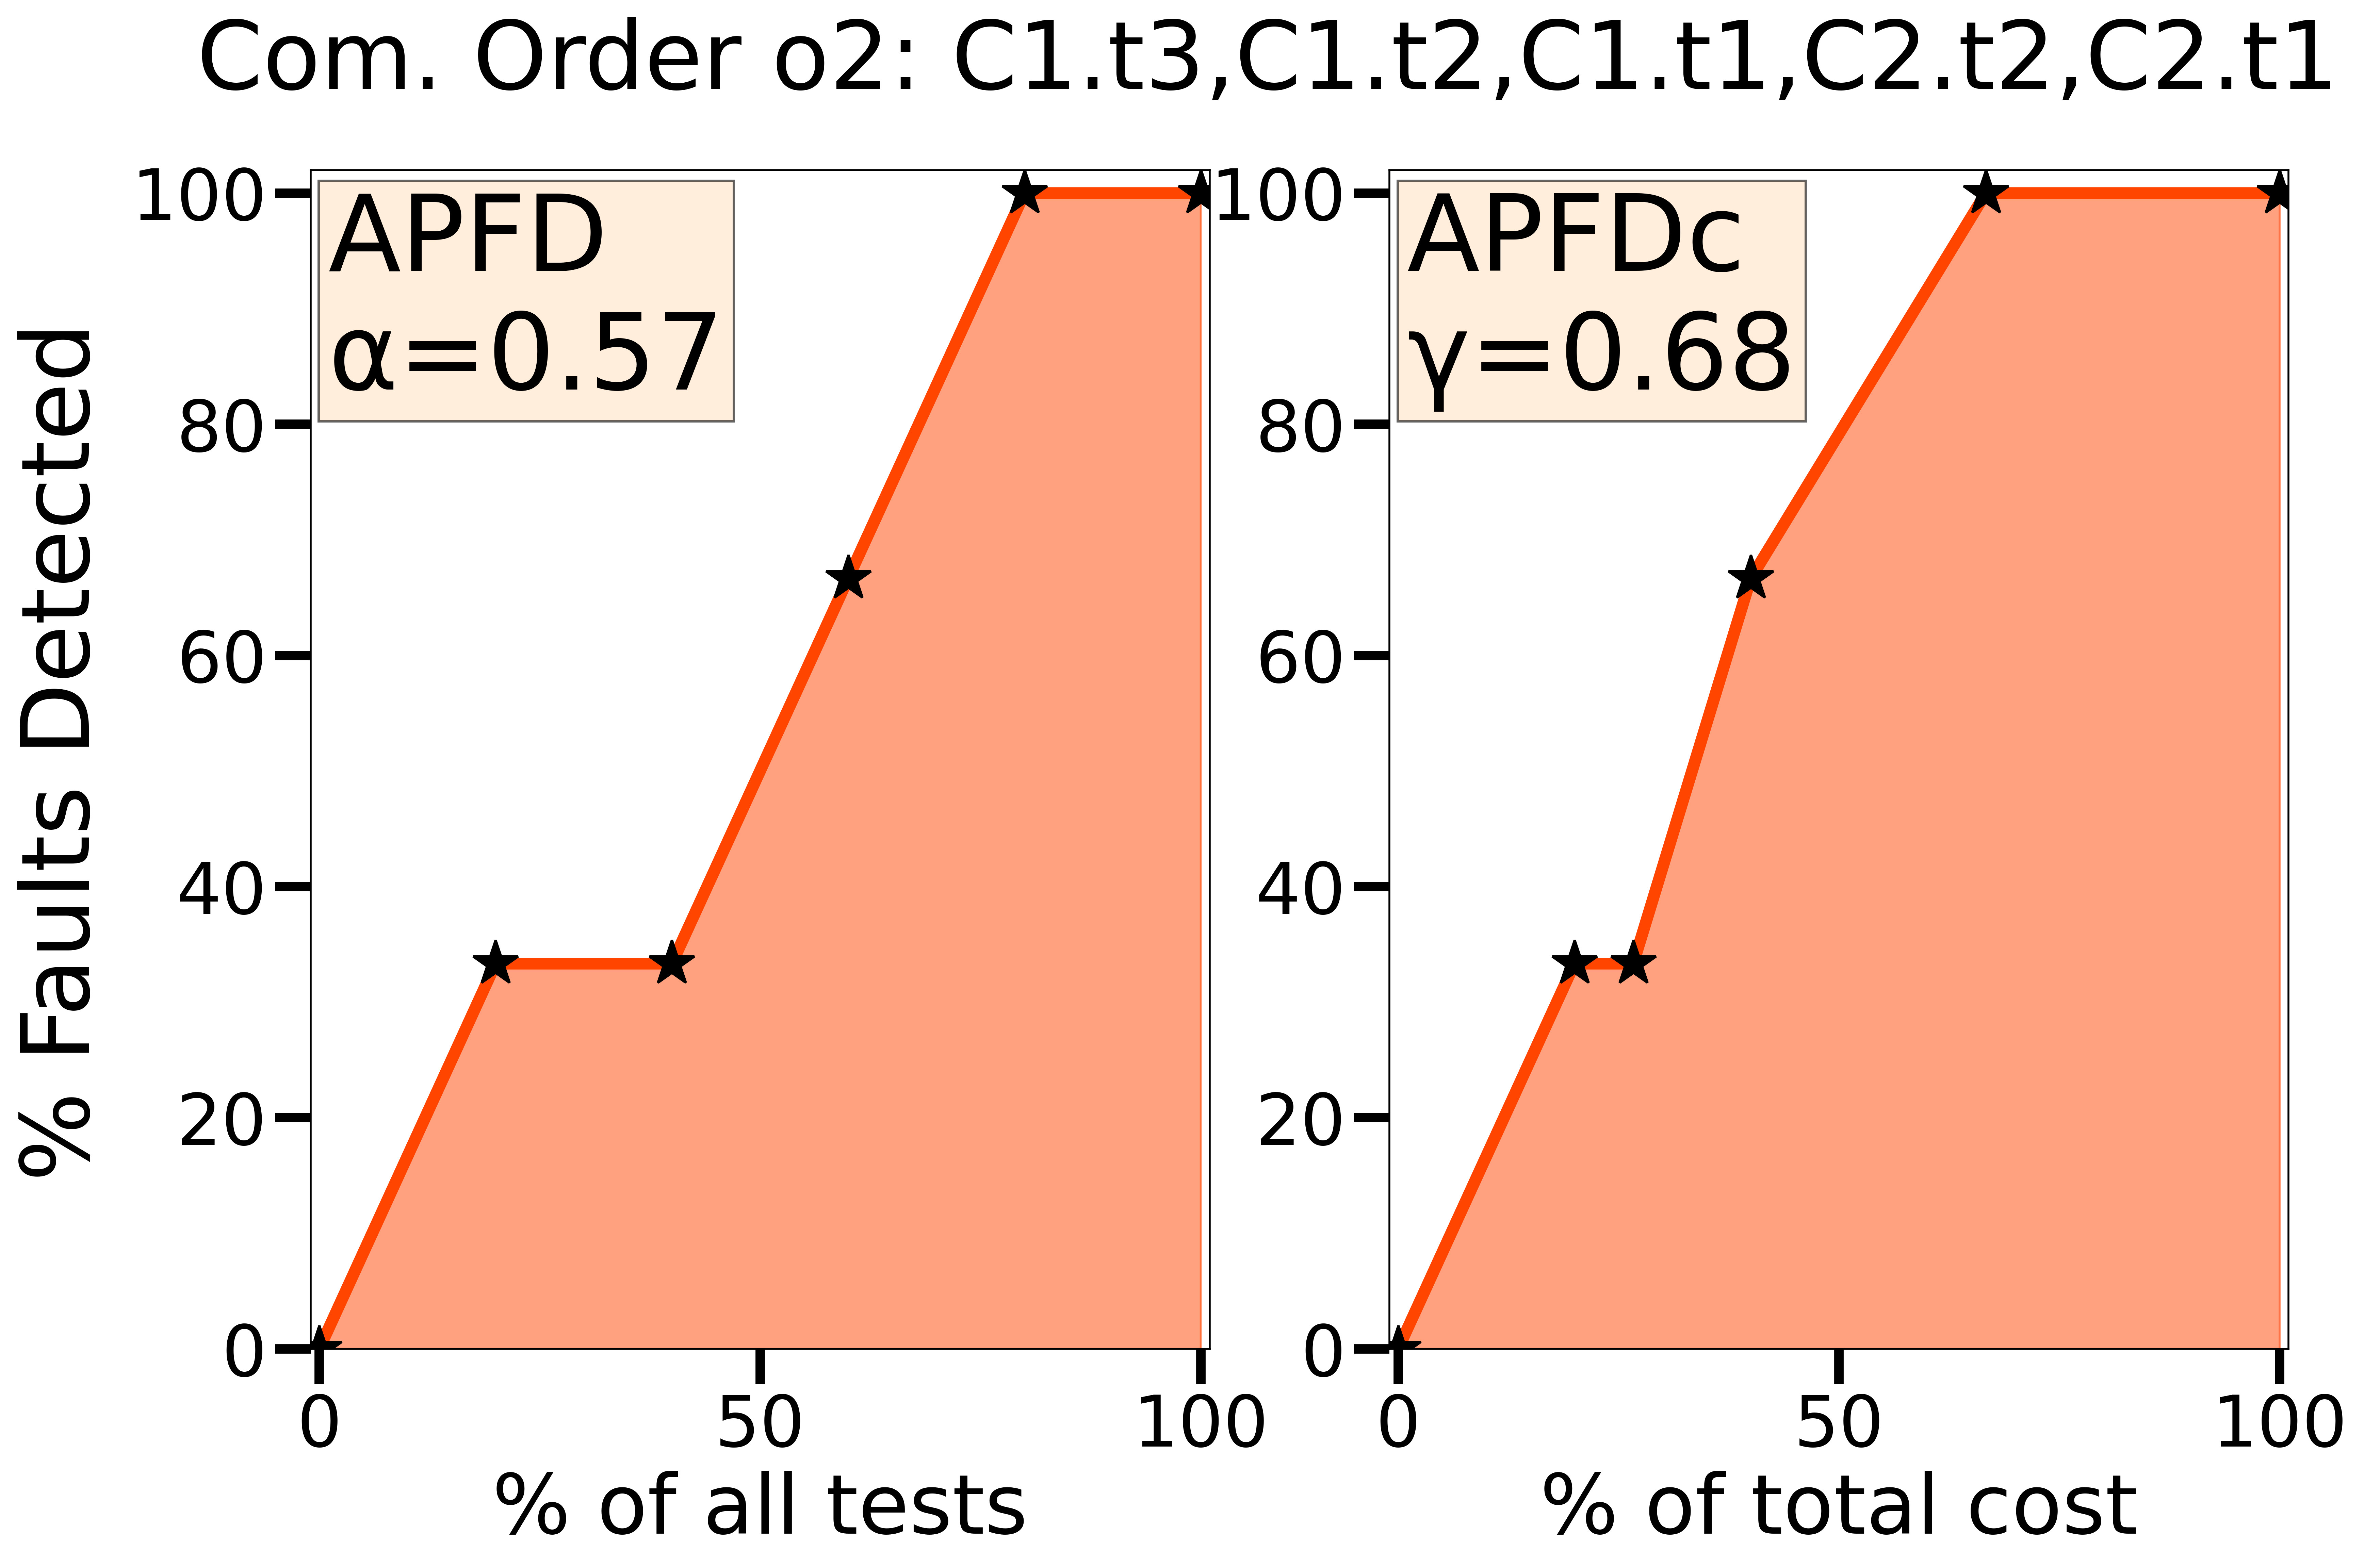
\includegraphics[width=\textwidth]{figures/3-2-1-5-4.png}
	\end{subfigure}
	\vspace{-1em}
	\caption{Example metrics for two orders (Com.\ is \compatible) for $n=5,m=3$; class C1 has 3 tests with costs $\langle40,20,60\rangle$, class C2 has 2 with $\langle100,80\rangle$; C1.t1 \detects fault F1; C1.t3 \detects F2; C2.t1 \detects F2 and F3; C2.t2 \detects F3.\label{fig:example}}
	\vspace{-0.2in}
\end{figure}

我们的记号很大程度上与提出\APFDFull{} (\APFD{})~\cite{rothermel2001prioritizing}和\APFDcFull{} (\APFDc{})~\cite{elbaum2001incorporating}的工作一致, 但我们显式地定义了 \mappingMatrix{}。
我们用$n$标记测试用例的数量,用$m$标记被这$n$个测试用例的其中一些检测到的缺陷数量。
我们用$M$标记一个\mappingMatrix{},也就是一个$n\times m$的布尔矩阵,其中$M_{j,i}=\textrm{true}$当且仅当测试用例$j$的失败可以\detects 缺陷$i$,并且其中每个缺陷都至少被一个测试用例检测(也就是说$\forall i.\exists j. M_{j,i}$)。
我们用$T$测试用例集中测试用例组成的一个集合.
我们将可以\detect{}缺陷$i$的测试用例的集合记做$T_i$,也就是说$T_i=\{j|M_{j,i}\}$。
总的来说,对于$i\ne i'$,$T_i$和$T_{i'}$可以有交集, 因为一个失败的测试用例可以\detect{}多个缺陷.
失败的总数记做$k$,也就是说$k=|\{j|\exists i. M_{j,i}\}|$,同时我们用$k_i$标记$T_i$集合的大小,即$k_i=|T_i|$。

对于一个执行次序$o$($T$的一个排列),我们用$<_o$来比较两个测试用例$t$和$t'$在该执行次序中的位置。$t<_o t'$表示$t$在$o$中先于$t'$执行,而$t\le_o t'$表示$t=t'$或$t<_o t'$。
我们用$t_{j}(o)$来表示$o$中的第$j$个测试用例。
我们用$TF_{i}(o)=\min_j M_{t_{j}(o),i}$标记$o$中第一个检测到故障$i$的测试用例的位置。
之前的工作~\cite{elbaum2001incorporating,rothermel2001prioritizing}定义了指标\APFD{}和\APFDc{}(使用符号$TF$而不是$\TF$)。
我们用$\APFD{}(o)$和$\APFDc{}(o)$分别表示执行次序$o$的 \APFD{}和\APFDc。
当从上下文可以清楚地知道所指的执行次序时,我们在$<_o$, $\le_o$, $t_{j}(o)$, $\TF_{i}(o)$, $\APFD{}(o)$, 和$\APFDc{}(o)$中省略$o$。

被使用最多的RTP指标是\APFD{}~\cite{rothermel2001prioritizing}。对一个执行次序$o$,\APFD{}定义如下。

\begin{mydefinition}[\APFD]
\APFDFull{}的定义为
\begin{equation}\label{definition_apfd}
    \APFD=1-\frac{\sum_{i=1}^m\TF_i}{nm}+\frac{1}{2n}
\end{equation}
\end{mydefinition}

如图~\ref{fig:example}中的两个例子所示,将检测到的缺陷百分比与执行的测试用例百分比作图,\APFD{}代表曲线下的面积。
图中每个点表示执行完若干测试用例后的情况,点之间的连线使得\APFD{}的均值/中位数具有良好的性质,并使其分布在一些情况下具有对称性(Section~\ref{sec:lit:review})。
\APFD{}的范围在0和1之间,更确切地说,在$1/(2n)$和$1-1/(2n)$之间。
较大的APFD{}表明一个测试用例平均而言较早检测到各个故障。

虽然\APFD{}有效地考虑了测试的数量,但 “代价感知型"指标\APFDc{}考虑了运行测试用例的代价~\cite{elbaum2001incorporating}。
运行测试用例的代价可以通过各种方式来衡量,但大多数工作都使用测试用例的运行时间。
我们用$\Cost{t}$表示一个测试用例$t$的代价(运行时间);一组测试$T$的总成本是$\Cost{T}=\sum_{t\in T}\Cost{t}$。

\begin{mydefinition}[\APFDc]
\APFDcFull{}的定义为
\begin{equation}\label{definition_apfdc}
    \APFDc=\frac{\sum_{i=1}^m\left(\sum_{j=\TF_i}^n\Cost{t_j}-\frac{1}{2}\Cost{t_{\TF_i}}\right)}{m\multi \Cost{T}}
\end{equation}
\end{mydefinition}

如\Figure~\ref{fig:example}所示,将检测到的缺陷百分比与测试用例集的总成本的百分比作图,\APFDc{}则代表曲线下的面积。
请注意,\APFD{}可以被看作是\APFDc{}在$\forall t,t’\in T.\Cost{t}=\Cost{t'}$情况下的一个特例。

在实践中,测试用例会被开发者分区,通常一个测试用例从属于一个\emph{\classes}——例如,JUnit~\cite{2021JUnit}中测试方法从属于测试类,Maven~\cite{2020Maven}中测试类属于测试模块,pytest~\cite{2021pytest}中测试函数属于测试文件--每个\class{}的测试一起运行。
我们之前的工作~\cite{wei2021probabilistic}将 \emph{\compatible{}}执行次序定义为每个\class{}的所有测试用例都是连续执行的执行次序。
我们用$T_\testClassInFormula$来表示$\testClassInFormula$\class{}中的测试用例的集合。
如果$\forall \testClassInFormula,j\le j'\le j''.t_{j}(o)\in T_\testClassInFormula\wedge t_{j''}(o)\in T_\testClassInFormula\Rightarrow t_{j'}(o)\in T_\testClassInFormula$,那么一个测试用例执行次序$o$是\compatible{}的。
例如,在\Figure~\ref{fig:example}中$o2$是\compatible{}的,而$o1$不是。

我们在不同的\emph{测试场景}中分析RTP技术,每个测试场景包含一个有$n$个测试用例、$m$个故障的测试用例集、\mappingMatrix{}、每个测试用例的代价以及对于$\consecutivetorders$每个测试的\class{}。
为了分析\compatible{}测试用例执行次序,我们引入一些新的符号来表示测试的\class{}。
我们用$T_{i,\testClassInFormula}=T_i\cap T_\testClassInFormula$来表示$\testClassInFormula$\class{}中能检测到$i$故障的测试集合。
我们用$\classSet$表示所有\class{}的集合,$\classSet_i$表示包含至少一个能检测到缺陷$i$的测试用例的\class{}的集合,即$\classSet_i=\{\testClassInFormula\in \classSet| T_{i,\testClassInFormula}\ne \emptyset\}$。
我们用$\classOfTest{t}$标记$t$所属的类,即$t\in T_{\classOfTest{t}}$。
\compatible{}测试用例执行次序的数量为$|\consecutivetorders|=|\classSet|!\prod_{\testClassInFormula\in \classSet}|T_\testClassInFormula|!$。

对于一组执行次序$S$,不管是$\alltorders$还是$\consecutivetorders$,RTP指标(\APFD{}或\APFDc{})的概率质量函数(\distribution{})是一个从指标值到其概率的函数$p$。$p(x)=\Prob{\mathrm{metric}=x}=\inlinefrac{|\{o\in S|\mathrm{metric}(o)=x\}|}{|S|}$。
所有先前的RTP工作都只显示了随机采样得到的随机RTP的样本分布,我们接下来推导一些\distributions{}。